\documentclass[a4paper]{article}
\usepackage{setspace}
\usepackage{url}
\usepackage{wrapfig}
%\usepackage{ieeefig}
%\usepackage{german}
%\usepackage{float}
%\usepackage{amsfonts}
\usepackage{graphicx}
%\usepackage{amsbsy}
%\usepackage{amsmath}
%\usepackage{theorem}
%\usepackage{dcolumn}
%\usepackage{enumerate}
%\usepackage[ansinew]{inputenc}

\setlength{\parindent}{0pt} \setlength{\parskip}{5pt plus 2pt minus 1pt}
\setlength{\textwidth}{16cm} \setlength{\textheight}{24.25cm}
\addtolength{\voffset}{-2.0cm}
\addtolength{\hoffset}{-2.25cm}
\doublespacing
%\singlespacing
%===========================================
%Credits: Format kindly provided by Niels Bernhardt
%===========================================
\begin{document}

\begin{center}  {\small 

									\textbf{Researcher :}Yogesh H. Kulkarni \hfill
									\textbf{Guides :} %Dr. Shailesh Deshpande and Dr. Mukund Kale 
								}
\end{center}


%\begin{center} Yogesh H. Kulkarni \end{center}

\begin{center} {\large \textbf{Doctoral Thesis Research Proposal}} \end{center}

\begin{center} 
	\textbf{} 
\end{center} \vspace{-6mm}

\begin{center} \textbf{} \end{center} \vskip5mm

%-------------------------------------------------------------------------------------------------------------------------------------------------------------------------------------%

\textbf{Provisional Thesis Title:}

Development of Feature Based Midsurface Creation Framework for Thin Wall Parts.

\vskip5mm

%-------------------------------------------------------------------------------------------------------------------------------------------------------------------------------------%

\textbf{Names of Supervisors/Advisors:}

  %Dr. Shailesh Deshpande and Dr. Mukund Kale

\vskip5mm

%-------------------------------------------------------------------------------------------------------------------------------------------------------------------------------------%

\textbf{Objectives/Aims:}

Develop a framework for generating connected-midsurfaces in feature-based modeling environment.
This framework is proposed to be based on non-manifold topology and will cater to features prominent in thin wall parts typically used in Sheet Metal Computer-Aided-Design (CAD) applications. Midsurface generated will be useful in further Computer-Aided-Engineering (CAE) processes. Proposed research work will include development of theoretical basis as well as software implementation.

\vskip5mm

%-------------------------------------------------------------------------------------------------------------------------------------------------------------------------------------%

\textbf{Problem Background}

Data provided by CAD models is often not suitable for CAE operations like Meshing. Some geometric-topological features are irrelevant and suppression of them does not harm accuracy of the analysis-result to a large extent, but in turn provide significant leverage in terms of processing time-space. Thus CAD models are often simplified-abstracted-idealized to suite needs of CAE analysis. One of the prominent simplification technique is called Midsurface (aka Medial Surface) which is highly suitable for thin wall parts prevelant in Plastics and Sheet Metal domain. Thin portions of the model are idealized to sheet surface along with thickness data to be modeled using shell elements. 

Midsurface techniques have been researched for past few decades. Major CAD-CAE softwares have Midsurfacing capability. Apart from CAE, midsurface (Figure ~\ref{MIDSURFRAM}) has found applications in Visualization, Animation, Model Simplification, Feature Recognition etc. 

In Midsurface related technologies, Researcher finds two broad categories of methodologies, one can be called as 'Medial Axis Transform (MAT)' methods and others can be called as 'Midsurface Abstraction(MA)' methods.

MAT is locus of the center of an inscribed disc of maximal diameter as it rolls around an object interior. The associated radius function gives the radius of the inscribed circle at every point on the skeleton, and makes the original 2D object recoverable from the medial axis. In 2D its called Medial Axis where as in 3D its called Medial Surface. 

\begin{wrapfigure}{r}{60mm}
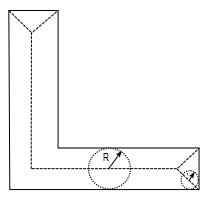
\includegraphics[scale=0.6]{../Common/images/MAT.jpg}
\caption{Medial Axis Transform \cite{Sheen2007}}
\label{MAT}
\end{wrapfigure}

Figure \ref{MAT} shows an example of the medial axis for a simple 2D profile \cite{Sheen2007}. 

Major drawback of this method is that it creates unnecessary branches and its shape is smaller than the original corresponding faces. Plus there is major issue of perturbations, meaning slight change in base geometry forces re computation of MAT and the result could very well be different than the original. 

MA(Figure ~\ref{MIDSURFRAM}) involves constructing the 3D mid-surface for a part model by connecting/sewing the mid-surface patches obtained for 'pairs of surfaces'. This requires a 'pairing strategy' that has thus far required human intervention. Connecting various mid-surface patches require 3D Boolean operations. 

\begin{wrapfigure}{r}{60mm}
\includegraphics[scale=0.4]{../Common/images//MIDSURF.jpg}
\caption{Midsurface Abstraction \cite{Ramanathan}}
\label{MIDSURFRAM}
\end{wrapfigure}

%\begin{wrapfigure}{r}{60mm}
%\includegraphics[scale=0.4]{MIDSURF.jpg}
%\caption{Midsurface Abstraction \cite{Sheen2007}}
%\label{MIDSURF}
%\end{wrapfigure}


The surface-pairing approach has benefits over other medial axis type techniques because the resultant geometry is cleaner and requires less reconstruction that those from medial axis approaches. However the surface pairing approach also has problems because it can be difficult to identify all of the surface pairs. 


Above mentioned techniques are based on \textbf{Extraction}, meaning, model is ready and then algorithm is applied  to extract midurface. \textbf{\textsl{Many a times due to complexity in recognizing forms, their interactions, same design-intent used while modeling part can not be applied to midsuface and thus midusface of part does not follow its form and connectivity}}\cite{Jxcad,Sheen2008} .

%\begin{wrapfigure}{r}{60mm}
%\includegraphics{MATMIDS.jpg}
%\caption{Midsurface Abstraction \cite{Sheen2008}}
%\label{MATMIDS}
%\end{wrapfigure}

Solution could be to create Midsurface while generating model.

In Features-based Solid Modeling, typically input feature-parameters are used to build tool-bodies and then part is built using direct or indirect boolean. Creating midsurface for individual tool bodies appears to be more deterministic problem than recognizing feature forms. With well-defined Boolean operation even correct midsuface interactions can be ensured. Researcher is of the opinion that this new approach can significantly improve midsuface connections than extraction methods. To the best of Researcher's knowledge and literature review done so far, there does not exist such system in reaserach as well as commerircial world.

There has been some work using M-Rep (Medial Representation similar to B-rep) which uses Medial entities as data model. But it has very basic data model and is mainly for Medical Visualization and not in domain of Feature-based Modelers\cite{Fletcher2004}. Another related effort generates midcurves in sketch and then sweeps to form midsurface \cite{Robinson2006}. This work is in Mix-Dimensional modeling, limited to sweep and does not seem to do feature interactions. 

Lee et al. \cite{Lee1995} suggested a conversion method from a sheet model to a solid model for the efficient solid modeling of thin-walled plastic or sheet metal parts. This method shows a great potential for degenerate solids in the representation of thin-walled parts. However, because this method adopts solid boundary representation, it is difficult to represent
the exact adjacency relations between topological entities in a sheet model, and to describe a mixture of wireframe and sheet objects that appear in the intermediate steps of sheet modeling operations. In order to overcome these problems, Lee et al. \cite{Lee2001} introduced a non-manifold boundary representation as a topological framework and proposed
a sheet thickening algorithm by presenting variations to a general non-manifold offset algorithm that is based on the mathematical definition of offsets. In addition, to facilitate sheet-modeling operations,  they provided a set of generalized Euler operators for non-manifold models as well as sheet modeling capabilities including adding, bending, and punching functions with two-dimensional curve editors. However, in these algorithms, all of the holes that lay
on thickness faces cannot be removed automatically, and topological irregularity of an offset face caused by self-intersection is not yet considered \cite{Lee2001}.

Thus research so far does not deal with the major problems of midsurface, that of connectivity and simplification. Gaps and extraneous features in midsuface render it useless for Meshing Operation. Proposed research is planning for improved and robust generation and connectivity of Midsurface\cite{Sheen2008}.

\vskip5mm

%-------------------------------------------------------------------------------------------------------------------------------------------------------------------------------------%

\textbf{Proposal-Point of Departure}

A \textbf{novel idea} is being proposed here, called \emph{Midsurface-On-Fly} (MoF). 
A non-manifold (surface-sheet) modeler will be proposed for Thin Wall modeling in which data-model will have all the information related to midsuface. The devised deta model will be able to switch itself to Solid model for purpose of calculating feature interaction and also visualization.

Making Midsurface as core data model will significantly improve connectivity and ensure more accurate analysis result.

\vskip5mm



%-------------------------------------------------------------------------------------------------------------------------------------------------------------------------------------%

\textbf{Schedule/Time line of Research:}

Reaserch is broken down into major chunks as follows:
\begin{itemize}
    \item \textbf{Semester 1:} In-depth literature survey.
    \item \textbf{Semester 2:} Mid curve generation methodology for Sketch
    \item \textbf{Semester 3:} Midusurface computation development for individual features
    \item \textbf{Semester 4:} Midsurface data formulation during feature interactions.
    \item \textbf{Semester 5:} Non-Manifold topology kernel development for midsurfaces.
    \item \textbf{Semester 6:} Implementation in-source or using APIs.
\end{itemize}

\vskip5mm


%-------------------------------------------------------------------------------------------------------------------------------------------------------------------------------------%


\bibliographystyle{plain}
\bibliography{../Common/MidsurfYogesh}
\end{document}
